\documentclass[11pt]{article}
% Shared preamble of the two technical papers (docs/paper). Compile with latexmk -pdf <paper>.tex
\usepackage[T1]{fontenc}
\usepackage[utf8]{inputenc}
\usepackage{lmodern}
\usepackage[a4paper,margin=25mm,headheight=14pt]{geometry}
\usepackage{microtype}
\usepackage{amsmath,amssymb,bm}
\usepackage{graphicx}
\usepackage{booktabs,tabularx,multirow}
\usepackage[detect-all,per-mode=symbol]{siunitx}
\usepackage{xcolor}
\usepackage{tikz}
\usetikzlibrary{arrows.meta,positioning,fit,calc,shapes.geometric,backgrounds}
\usepackage{caption,subcaption}
\usepackage{enumitem}
\usepackage{algorithm}
\usepackage{algpseudocode}
\usepackage{authblk}
\usepackage{fancyhdr}
\usepackage[numbers,sort&compress]{natbib}
\usepackage[colorlinks=true,linkcolor=blue!50!black,citecolor=blue!50!black,urlcolor=blue!50!black]{hyperref}
\usepackage[capitalise,noabbrev]{cleveref}

\definecolor{lrred}{HTML}{C8102E}
\definecolor{cA}{HTML}{2A78D6}
\definecolor{cB}{HTML}{EB6834}
\definecolor{cC}{HTML}{1BAF7A}
\definecolor{boxbg}{HTML}{F3F4F6}

\captionsetup{font=small,labelfont=bf,margin=4pt}
\setlist{itemsep=2pt,topsep=3pt}
\sisetup{group-minimum-digits=4}
\numberwithin{equation}{section}

\pagestyle{fancy}
\fancyhf{}
\renewcommand{\headrulewidth}{0.3pt}
\fancyfoot[C]{\thepage}

\newcommand{\code}[1]{\texttt{\small #1}}
\newcommand{\vect}[1]{\bm{#1}}
\renewcommand{\Affilfont}{\small\itshape}

% TikZ styles for the block diagrams
\tikzset{
  blk/.style={draw=black!60, fill=boxbg, rounded corners=2pt, align=center, font=\footnotesize, inner sep=4pt, minimum height=8mm},
  grp/.style={draw=black!35, dashed, rounded corners=3pt, inner sep=5pt},
  grplab/.style={font=\scriptsize\itshape, text=black!60},
  arr/.style={-{Stealth[length=2mm]}, semithick, black!70},
  darr/.style={{Stealth[length=2mm]}-{Stealth[length=2mm]}, semithick, black!70},
}


\fancyhead[L]{\small fsg-dv-sim: a shared-model simulator for the LR26 driverless vehicle}
\fancyhead[R]{\small Lions Racing Team}

\title{\textbf{fsg-dv-sim: A Shared-Model Simulation Environment\\for the Lions Racing LR26 Formula Student Driverless Vehicle}\\[4pt]
\large Vehicle dynamics, sensor models, perception, SLAM, control and the Isaac Sim co-simulation}
% Authors: edit as appropriate.
\author{Lions Racing Team -- Driverless Division}
\affil{Formula Student Germany}
\date{Technical report, November 2026}

\begin{document}
\maketitle
\thispagestyle{fancy}

\begin{abstract}
\noindent
This report describes \emph{fsg-dv-sim}, the simulation environment of the Lions Racing LR26 driverless car. The
design rests on one principle: every behavioural model exists once and is shared by every part of the toolchain. The
vehicle dynamics, the autonomous-system state machine, timing, penalties and the proprioceptive sensors live in a
pure Python/NumPy core (\code{fsdsim}). That core drives three front ends: a GPU-free ``lite'' ROS~2 backend, an
NVIDIA Isaac Sim backend with ray-traced LiDAR and camera rendering, and a batched array version for reinforcement
learning on thousands of vehicle specifications at once. The planar vehicle model is a dynamic single-track model,
blended into a kinematic model at low speed. In its \emph{performance} mode, every tyre, aerodynamic, powertrain and
brake limit comes from a line-by-line port of the Performance department's quasi-steady-state lap time simulation
(LapSim). The driverless simulator and the lap time tool therefore share a single parameter file. On top of the
plant we describe:
\begin{itemize}
  \item analytic models of the Ouster OS1-64 LiDAR, the ZED~2i stereo camera, the IMU, the GNSS and the wheel
        sensors, with fault injection;
  \item a ground-truth-free perception chain: LiDAR cone detection, camera fusion and a landmark SLAM with
        closed-form rigid alignment;
  \item a reference driver (pure pursuit with speed targets from the LapSim model) and two learned longitudinal
        controllers;
  \item a TCP co-simulation link between Isaac Sim on Windows and ROS~2 in WSL, together with the timing defects
        found and removed on the team computer.
\end{itemize}
The test suite has 319 tests. In closed loop, the reference driver finishes every Formula Student
event without penalties. With LiDAR--camera fusion and SLAM, an autocross run maps all 113 cones with
\SI{0.074}{m} rms position error and a mean pose error of \SI{0.057}{m}. In Isaac Sim, a ten-lap trackdrive on the
racing line is driven at \SI{18.85}{s} per lap without penalties.
\end{abstract}

\noindent\textbf{Keywords:} autonomous racing; Formula Student Driverless; vehicle simulation; digital twin; sensor
simulation; SLAM; pure pursuit; reinforcement learning; Isaac Sim; ROS~2.

\tableofcontents
\newpage

%=====================================================================================================
\section{Introduction}
%=====================================================================================================
Formula Student Driverless (FSD) asks student teams to build a car that completes four dynamic disciplines with no
human driver: acceleration, skidpad, autocross and trackdrive. The software stack has to perceive cones, localise,
plan a path and control the car at the limit of adhesion. Development time on the real car is scarce, and the real
car is often not available at all. A simulator is therefore the main development platform of a driverless team.
It is only useful if it predicts what the real stack will see and how the real car will respond.

Teams typically run into three problems with simulators. First, the vehicle model of the simulator and the lap time
model of the vehicle-dynamics group drift apart, so the driverless and performance numbers cannot be compared.
Second, photorealistic simulators (game engines, Isaac Sim) bring their own physics, which must be tuned again and
which ties every test to a GPU. Third, the interface to the autonomy stack differs between simulator and car, so
code paths that only run on the car are never tested.

fsg-dv-sim addresses these problems with four design rules (\cref{sec:arch}):
\begin{enumerate}
  \item \textbf{One interface for simulator and car.} The stack only sees ROS~2 topics whose types, frames and
        names match the car's drivers (ouster-ros point fields, the ZED wrapper topic layout, the FSD CAN state
        codes).
  \item \textbf{One source of truth for behaviour.} Dynamics, rules and proprioceptive sensors live in
        \code{fsdsim}. A renderer only decides how LiDAR and camera data are produced.
  \item \textbf{Testable without a GPU.} The core is pure Python/NumPy, so unit and closed-loop regression tests
        run anywhere.
  \item \textbf{Everything identifiable is a parameter.} Vehicle, sensors, events and rules are YAML or the LapSim
        parameter file. That turns the step from simulator to digital twin into a data problem.
\end{enumerate}

\paragraph{Contributions.}
\begin{itemize}
  \item A vehicle model whose force limits are the Performance department's LapSim model, so that the simulator,
        the lap time simulation and MATLAB share one parameter file (\cref{sec:vehicle}).
  \item Sensor models that reproduce the data layout and the main error mechanisms of the car's sensors, including
        LiDAR motion distortion and sensor faults (\cref{sec:sensors}).
  \item A ground-truth-free perception and SLAM chain, plus the timing analysis that made it work against Isaac
        Sim's rendered sensors (\cref{sec:perception,sec:isaac}).
  \item A reference driver whose speed targets come from the car's own QSS model, a racing-line optimiser, and two
        learned longitudinal controllers, one per setup and one universal across setups (\cref{sec:control}).
  \item A verification strategy with 319 automated tests and a 33-case closed-loop regression
        (\cref{sec:verification}).
\end{itemize}
The companion report~\cite{perflab} describes the stand-alone lap time simulation (the Performance Lab). That
report covers the quasi-steady-state solver this simulator uses in detail.

%=====================================================================================================
\section{Related work}\label{sec:related}
%=====================================================================================================
Several FSD teams have published simulators. FSSIM by AMZ Racing~\cite{fssim} couples a dynamic bicycle model to
Gazebo. The AMZ full-system paper~\cite{kabzan2020} describes the blend of a kinematic and a dynamic single-track
model at low speed, which we adopt. Single-track models and their limits are textbook material~\cite{rajamani2012};
the tyre force shape follows Pacejka's Magic Formula~\cite{pacejka2012}. Quasi-steady-state (QSS) lap time
simulation goes back to point-mass and ``apex speed'' methods~\cite{siegler2000,brayshaw2005}. Minimum-time optimal
control is the reference for transient strategies~\cite{casanova2000}. Minimum-curvature racing lines with
quadratic programming are standard in autonomous racing~\cite{heilmeier2020}. Our racing-line formulation is an
independent bounded least-squares variant, not derived from that code.

Pure pursuit~\cite{coulter1992} remains the most common FSD path tracker because of its robustness at low
computational cost. Cone detection from LiDAR by ground removal and clustering, and from the camera with CNN
detectors, is described in~\cite{dhall2019,kabzan2020}. Our camera detector uses Ultralytics YOLO~\cite{yolo11}.
The landmark SLAM uses the closed-form rigid alignment of Kabsch~\cite{kabsch1976}. For learning, we use DAgger
imitation~\cite{ross2011}, OpenAI evolution strategies~\cite{salimans2017} and PPO~\cite{schulman2017} with
generalised advantage estimation~\cite{schulman2016}. The batched environment follows the GPU-parallel simulation
approach of Isaac Gym and Isaac Lab/Orbit~\cite{makoviychuk2021,mittal2023}. ROS~2~\cite{macenski2022} is the
middleware.

%=====================================================================================================
\section{System architecture}\label{sec:arch}
%=====================================================================================================
\Cref{fig:arch} shows the main components. \code{fsdsim} is the simulation core. \code{fsd\_sim\_bridge} contains
the ROS~2 nodes. Only \code{ros\_interface.py} turns simulator events into ROS messages, and the lite node and the
Isaac relay both use it. The dashboard, a launcher and the Performance tools sit on the same topics, so they work
the same against the simulator, a bag replay or the real car.

\begin{figure}[t]
\centering
\resizebox{\textwidth}{!}{%
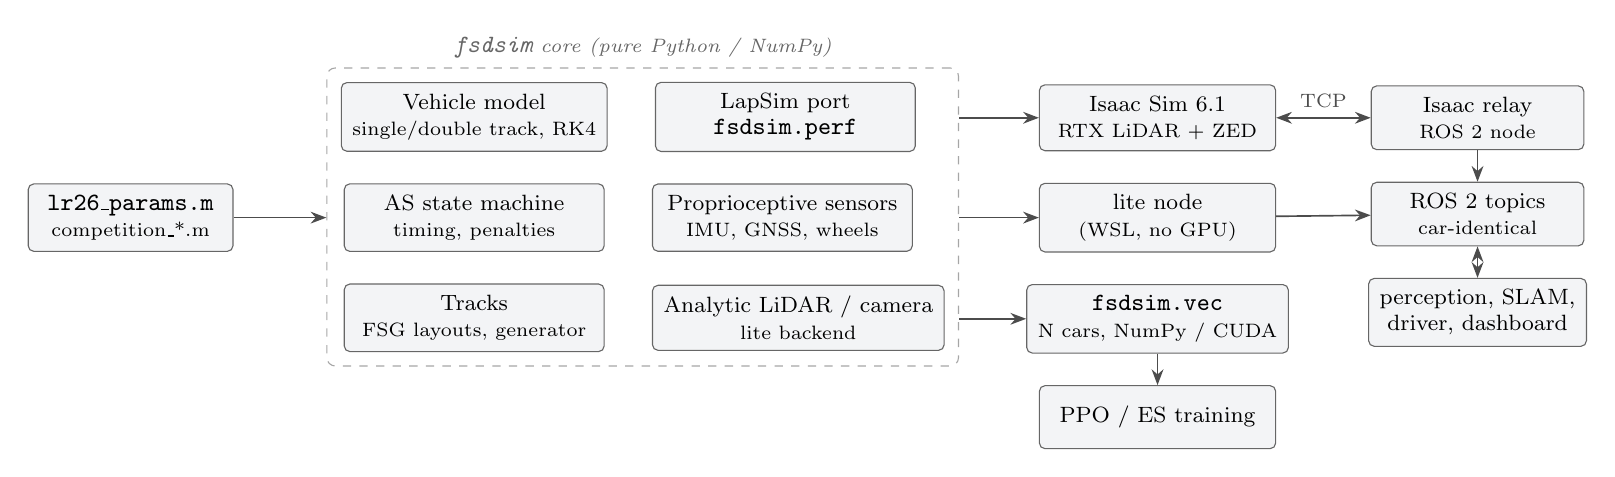
\begin{tikzpicture}[node distance=4mm and 6mm]
  % core
  \node[blk, minimum width=33mm] (dyn) {Vehicle model\\\scriptsize single/double track, RK4};
  \node[blk, right=of dyn, minimum width=33mm] (perf) {LapSim port\\\scriptsize \code{fsdsim.perf}};
  \node[blk, below=of dyn, minimum width=33mm] (mis) {AS state machine\\\scriptsize timing, penalties};
  \node[blk, right=of mis, minimum width=33mm] (sen) {Proprioceptive sensors\\\scriptsize IMU, GNSS, wheels};
  \node[blk, below=of mis, minimum width=33mm] (trk) {Tracks\\\scriptsize FSG layouts, generator};
  \node[blk, right=of trk, minimum width=33mm] (lid) {Analytic LiDAR / camera\\\scriptsize lite backend};
  \node[grp, fit=(dyn)(perf)(mis)(sen)(trk)(lid), label={[grplab]above:\code{fsdsim} core (pure Python / NumPy)}] (core) {};
  \node[blk, left=14mm of mis, minimum width=26mm] (lm) {\code{lr26\_params.m}\\\scriptsize competition\_*.m};
  \draw[arr] (lm) -- (core.west |- lm);
  % backends
  \node[blk, right=16mm of sen, minimum width=30mm] (lite) {lite node\\\scriptsize (WSL, no GPU)};
  \node[blk, above=of lite, minimum width=30mm] (isaac) {Isaac Sim 6.1\\\scriptsize RTX LiDAR + ZED};
  \node[blk, below=of lite, minimum width=30mm] (vec) {\code{fsdsim.vec}\\\scriptsize N cars, NumPy / CUDA};
  \draw[arr] (core.east |- isaac) -- (isaac);
  \draw[arr] (core.east |- lite) -- (lite);
  \draw[arr] (core.east |- vec) -- (vec);
  % ROS side
  \node[blk, right=12mm of isaac, minimum width=27mm] (relay) {Isaac relay\\\scriptsize ROS 2 node};
  \draw[darr] (isaac) -- node[above, font=\scriptsize]{TCP} (relay);
  \node[blk, below=of relay, minimum width=27mm] (ros) {ROS 2 topics\\\scriptsize car-identical};
  \draw[arr] (relay) -- (ros); \draw[arr] (lite) -- (ros);
  \node[blk, below=of ros, minimum width=27mm] (stack) {perception, SLAM,\\driver, dashboard};
  \draw[darr] (ros) -- (stack);
  \node[blk, below=of vec, minimum width=30mm] (ppo) {PPO / ES training};
  \draw[arr] (vec) -- (ppo);
\end{tikzpicture}}
\caption{Architecture. The core is shared by all backends. The LapSim parameter file is read directly, so the
lap time simulation and the driverless simulator use the same car. Only the renderer differs between the
backends.}
\label{fig:arch}
\end{figure}

\subsection{Simulation loop}
\code{Simulation.step(dt)} advances the world by one control period. Inside, physics is sub-stepped at
\SI{500}{Hz}, and every sub-step runs the following sequence:
\begin{enumerate}
  \item The autonomous-system auto sequence runs: mission select, ASMS on, then ``Go'' after the ready time once
        the control stream is alive.
  \item The control watchdog is checked. In AS Driving, a command older than \SI{1}{s} triggers AS Emergency.
  \item A brake override is applied: holding brakes (\SI{5}{m/s^2}) in Off, Ready and Finished; EBS
        (\SI{10}{m/s^2}) in Emergency.
  \item The vehicle model is integrated (RK4).
  \item The footprint is tested against every cone base circle. A hit knocks the cone and adds \SI{2}{s}.
  \item The mission is updated:
        \begin{itemize}
          \item timing-line crossings, interpolated to sub-step time;
          \item laps, off-course (\SI{10}{s}) and leaving the track;
          \item standstill (below \SI{0.1}{m/s} for \SI{1}{s}) leading to AS Finished.
        \end{itemize}
  \item Every sensor is sampled when due, each on its own rate scheduler.
\end{enumerate}
The outputs are plain dictionaries (\emph{events}):
\begin{itemize}
  \item \code{imu}, \code{gnss}, \code{vehicle\_sensors}, \code{lidar}, \code{camera\_detections};
  \item \code{as\_status}, \code{ground\_truth}, \code{cones}, \code{track}.
\end{itemize}
They contain no ROS types, which keeps the core usable from Isaac Sim's Python, the training code and the tests.

\subsection{Backends and time}
The \textbf{lite backend} runs the core inside a ROS~2 node and publishes \code{/clock}.

The \textbf{Isaac backend} runs the core inside Isaac Sim's Python process on Windows. It does not let PhysX
simulate the car: the car prim is moved every rendered frame from the \code{fsdsim} state (a kinematic chassis).
This keeps the behaviour identical between backends and avoids tuning a second vehicle model. RTX sensors
ray-trace the scene at render time, so they are not affected by how the chassis is moved.

\code{fsdsim} is the time authority. Before each rendered frame it is advanced to that frame's time, so events,
LiDAR scans and images share one time base. The relay publishes it as \code{/clock}, and every other node runs with
\code{use\_sim\_time}.

%=====================================================================================================
\section{Vehicle model}\label{sec:vehicle}
%=====================================================================================================
\subsection{State, inputs and kinematics}
The state is
\begin{equation}
\vect{x} = [X,\;Y,\;\psi,\;v_x,\;v_y,\;r,\;\delta,\;a]^\top,
\end{equation}
with the position and yaw $(X,Y,\psi)$ in the map frame, the body-frame velocities $v_x, v_y$ at the centre of
gravity (CoG), the yaw rate $r$, the road-wheel angle $\delta$ and the realised longitudinal acceleration request
$a$. The inputs are the steering request $\delta_c$ and the signed acceleration request $a_c$. The position
evolves as
\begin{equation}
\dot X = v_x\cos\psi - v_y\sin\psi,\qquad \dot Y = v_x\sin\psi + v_y\cos\psi,\qquad \dot\psi = r .
\end{equation}

\paragraph{Actuators.} Steering is a first-order lag with a rate limit; the acceleration request is a first-order
lag:
\begin{equation}
\dot\delta = \operatorname{sat}_{\pm\dot\delta_{\max}}\!\left(\frac{\delta_c-\delta}{\tau_\delta}\right),\qquad
\dot a = \frac{a_c - a}{\tau_a},
\end{equation}
with $\tau_\delta=\SI{0.05}{s}$, $\tau_a=\SI{0.06}{s}$, $\dot\delta_{\max}=\SI{1.5}{rad/s}$ and
$|\delta|\le\SI{0.42}{rad}$.

\subsection{Dynamic single-track model}
The slip angles at the axles are
\begin{equation}
\alpha_f = \delta - \operatorname{atan2}(v_y + l_f r,\; \tilde v_x),\qquad
\alpha_r = -\operatorname{atan2}(v_y - l_r r,\; \tilde v_x),\qquad \tilde v_x = \max(v_x, \SI{0.5}{m/s}).
\end{equation}
With axle forces $F_{x\{f,r\}}, F_{y\{f,r\}}$, drag $F_D$ and rolling resistance $F_R$, the equations of motion
are
\begin{align}
m_x(\dot v_x - v_y r) &= F_{xr} + F_{xf}\cos\delta - F_{yf}\sin\delta - F_D - F_R, \label{eq:vx}\\
m(\dot v_y + v_x r) &= F_{yr} + F_{xf}\sin\delta + F_{yf}\cos\delta,\\
I_z \dot r &= l_f\,(F_{yf}\cos\delta + F_{xf}\sin\delta) - l_r F_{yr},
\end{align}
where $m_x = e_i\,m$ includes the rotating-mass factor $e_i$ and $I_z=\SI{120}{kg\,m^2}$ (LapSim has no yaw
inertia).

\paragraph{Low-speed kinematic blend.} The dynamic model is singular as $v_x\to 0$. Below a blend window
$[v_{lo}, v_{hi}] = [3, 5]\,\si{m/s}$, the derivatives of a kinematic single-track model take over,
\begin{equation}
\dot v_x^{kin} = \frac{F_{xf}+F_{xr}-F_D-F_R}{m_x},\quad
\dot v_y^{kin} = (\dot\delta v_x + \delta \dot v_x^{kin})\frac{l_r}{L},\quad
\dot r^{kin} = \frac{\dot\delta v_x + \delta \dot v_x^{kin}}{L},
\end{equation}
mixed with weight
$\lambda = \operatorname{clip}\big((\lVert\vect v\rVert - v_{lo})/(v_{hi}-v_{lo}), 0, 1\big)$ as
$\dot{\vect z} = \lambda\,\dot{\vect z}^{dyn} + (1-\lambda)\,\dot{\vect z}^{kin}$ for $\vect z = (v_x, v_y, r)$. After each sub-step, $v_y$ and
$r$ are relaxed towards their kinematic values with the same weight, and reversing is prevented. This is the AMZ
approach~\cite{kabzan2020}.

\paragraph{Integration.} Classical fourth-order Runge--Kutta with sub-steps $h\le\SI{2}{ms}$. Inputs are held over
a control period.

\subsection{Force limits from the LapSim model (performance mode)}\label{sec:perfmode}
In the \emph{performance} mode, every force limit comes from the port of the LR26 LapSim~\cite{perflab}. The
quantities are evaluated with the body accelerations $(a_x, a_y)$ of the previous evaluation (quasi-static load
transfer, as in LapSim).

\paragraph{Wheel loads.} With wheelbase $L=l_f+l_r$, CoG height $h$, track widths $s_f, s_r$ and downforce
$F_{DF} = \tfrac12\rho c_z A\,\eta_{aero} v^2$ split by the front aero balance $k_f$:
\begin{align}
F_{z,f} &= \frac{m g l_r}{L} + k_f F_{DF} - \frac{m a_x h}{L}, &
F_{z,r} &= \frac{m g l_f}{L} + (1-k_f) F_{DF} + \frac{m a_x h}{L},\\
\Delta F_{y,f} &= \frac{m a_y h}{s_f}\frac{l_r}{L}, &
\Delta F_{y,r} &= \frac{m a_y h}{s_r}\frac{l_f}{L},
\end{align}
and the four wheel loads are $F_{z,f}/2 \mp \Delta F_{y,f}$ and $F_{z,r}/2 \mp \Delta F_{y,r}$, clipped at zero.

\paragraph{Tyre potentials.} The tyre potentials per wheel $i$ are load sensitive,
\begin{equation}
p_{x,i} = F_{z,i}\big(\mu_x + \tfrac{\partial\mu_x}{\partial F_z}(F_{z,i}-F_{z0})\big),\qquad
p_{y,i} = F_{z,i}\big(\mu_y + \tfrac{\partial\mu_y}{\partial F_z}(F_{z,i}-F_{z0})\big),
\end{equation}
and they are summed per axle to $p_x^{ax}$, $p_y^{ax}$.

\paragraph{Lateral force.} The lateral axle force is the potential times a Magic-Formula shape with unit
peak~\cite{pacejka2012},
\begin{equation}
F_y = p_y^{ax}\,S(\alpha),\qquad S(\alpha) = \sin\!\big(C\arctan(B\alpha - E(B\alpha-\arctan B\alpha))\big),
\label{eq:shape}
\end{equation}
with $B=11$, $C=1.45$, $E=0.3$. For $C>1$ the maximum is exactly $1$, reached at $\alpha^\star = \ang{11.5}$
(\cref{fig:tyre}).

\paragraph{Cornering priority (friction ellipse).} As in LapSim, cornering has priority, and drive and brake
forces may only use what the friction ellipse leaves:
\begin{equation}
F_{x,\mathrm{rem}} = p_x^{ax}\,\big(1 - u^{e}\big)^{1/e},\qquad u = \begin{cases}\min(|S(\alpha)|,1) & |\alpha|<\alpha^\star\\ 1 & |\alpha|\ge\alpha^\star\end{cases}
\label{eq:rem}
\end{equation}
with the ellipse exponent $e=2$. Past the peak slip angle the tyre counts as fully used. Otherwise the falling
branch of the Magic Formula would free longitudinal grip and spin the car. On the real car, this is the job of
traction control and ABS.

\begin{figure}[t]
\centering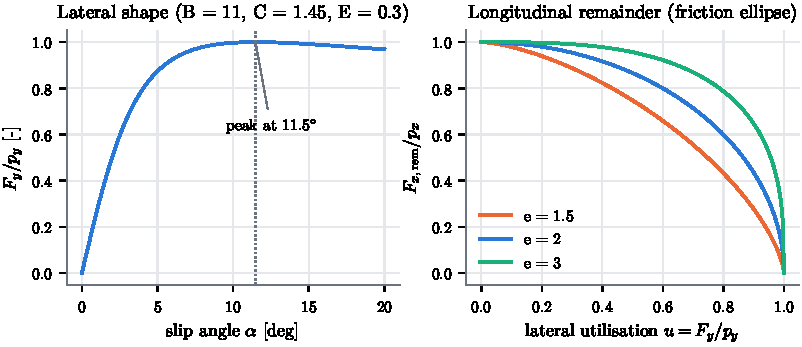
\includegraphics[width=\textwidth]{figures/dv_tyre.pdf}
\caption{Tyre model of the performance mode. Left: lateral shape $S(\alpha)$ of \cref{eq:shape}, scaled by the
LapSim axle potential. Right: longitudinal force left by the friction ellipse, \cref{eq:rem}, for three exponents
(LR26: $e=2$).}
\label{fig:tyre}
\end{figure}

\paragraph{Powertrain.} With wheel radius $r_w = c_{ref}/2\pi$, gear ratio $i$, motor speed
$\omega_m = v\,i/r_w$ and power limit $P$:
\begin{equation}
T = \min\!\left(T_{mot}, \frac{P}{\omega_m}\right),\quad F_{set} = \frac{T\,i\,\eta_g}{r_w}\;\;(0 \text{ above } v_{\max}=\tfrac{2\pi n_{\max}}{60}\tfrac{r_w}{i}),\quad
F_{cap} = \frac{P\,\eta_g}{v}.
\end{equation}
For rear-wheel drive, the requested drive force $F = m_x a$ becomes
$F_{xr} = \min(F, F_{set}, F_{x,\mathrm{rem},r})$, scaled down proportionally if the sum exceeds $F_{cap}$. For
all-wheel drive, half the request goes to each axle with the same limits. The model reports which limit is active
(power, traction, motor).

\paragraph{Brakes.} With a fixed front bias $b$, the request $B=-m_x a$ is split
$(bB, (1-b)B)$ and limited per axle by $F_{x,\mathrm{rem}}$. With the default ideal balance, it is split in
proportion to the axle remainders.

\paragraph{Resistance.} Drag $F_D = \tfrac12\rho c_w A\,\eta_{aero} v^2$ and rolling resistance
$F_R = f_r (mg + F_{DF})\tanh(v/0.2)$. The $\tanh$ only removes the discontinuity at standstill.

\subsection{Double-track handling}
With \code{handling: double\_track}, slip angle, load (longitudinal and lateral transfer), potential and force are
evaluated per wheel. Drive is shared per wheel with per-wheel traction control (one inverter per side), and brakes
use equal pressure left and right with per-wheel ABS. Summing the body forces gives the yaw moment
$M_z=\sum_i (x_i F_{y,i}^b - y_i F_{x,i}^b)$, so unequal left/right forces turn the car. The default single-track
mode keeps the LapSim axle forces, so lap times stay consistent with the Performance model. Double track changes
the skidpad time by about \SI{0.01}{s} and exists for work on yaw control and torque vectoring.

\subsection{Chassis attitude, wheel slip and energy}
Roll $\phi$, pitch $\theta$ and heave $z$ of the sprung mass do not feed back into the planar motion (the
relevant load transfer is already in the wheel loads), but they tilt what the sensors see. Each follows a
second-order response towards a steady state, e.g.
\begin{equation}
\ddot\phi + 2\zeta\omega_\phi\dot\phi + \omega_\phi^2(\phi - k_\phi a_y/g) = 0,
\end{equation}
with roll gradient $k_\phi=\SI{0.7}{\degree/g}$, pitch gradient $\SI{0.45}{\degree/g}$, natural frequencies
3.2/3.6/\SI{3.4}{Hz} and damping $\zeta=0.65$. The heave target is $-F_{DF}/K_{ride}$. These values are typical
Formula Student values, not yet measured on the LR26.

Longitudinal wheel slip comes from inverting $F_x = p_x\sin(C_s\arctan(B_s\kappa))$ ($B_s=12$, $C_s=1.5$). The
wheel-speed sensors therefore over-read under traction and under-read under braking.

The battery power, with recuperation limited to $P_{regen}$ and weighted by $\eta_{regen}$, is
\begin{equation}
P_{batt} = \begin{cases} F_x v / (\eta_g \eta_m(T,n)) & F_x v \ge 0\\ -\min(|F_x v|, P_{regen})\,\eta_{regen} & \text{otherwise}\end{cases}
\end{equation}
where $\eta_m$ is a constant or a motor-efficiency map from car logs~\cite{perflab}. Integrating $P_{batt}$ gives
the energy meter.

\subsection{LR26 parameters}
\Cref{tab:params} lists the main parameters. The LapSim values are read from \code{lr26\_params.m} at start-up; the
simulator-only values are in \code{vehicle.yaml}.

\begin{table}[t]
\centering\small
\caption{Main LR26 parameters used by the simulator (LapSim set, documentation v2.0 Table 3.1, and simulator-only
entries).}
\label{tab:params}
\setlength{\tabcolsep}{4pt}\footnotesize
\begin{tabular}{@{}llr|llr@{}}
\toprule
Mass incl. driver $m$ & kg & 284 & Gear ratio $i$ & -- & 14.5\\
CoG to front / rear axle $l_f,l_r$ & m & 0.851 / 0.754 & Peak motor torque per axle $T_{mot}$ & Nm & 38\\
CoG height $h$ & m & 0.265 & Max motor speed $n_{\max}$ & rpm & 21\,000\\
Track width $s_f=s_r$ & m & 1.226 & Power limit $P_{\max}$ & kW & 80\\
Friction $\mu_x / \mu_y$ & -- & 1.43 / 1.64 & Endurance power cap & kW & 18\\
Load sensitivity $\partial\mu_x/\partial F_z$ & 1/N & $-2.28\times10^{-5}$ & Gearbox efficiency $\eta_g$ & -- & 0.95\\
Load sensitivity $\partial\mu_y/\partial F_z$ & 1/N & $-1.47\times10^{-4}$ & Motor efficiency $\eta_m$ & -- & 0.90\\
Drag / downforce coefficient $c_w,c_z$ & -- & 1.38 / 4.15 & Tyre circumference $c_{ref}$ & m & 1.57\\
Frontal area $A$, aero efficiency & m$^2$, -- & 1.044, 0.80 & Rolling resistance $f_r$ & -- & 0.005\\
Front aero balance $k_f$ & -- & 0.485 & Yaw inertia $I_z$ (sim) & kg\,m$^2$ & 120\\
Air density $\rho$ & kg/m$^3$ & 1.18 & Max steering angle (sim) & rad & 0.42\\
\bottomrule
\end{tabular}
\end{table}

%=====================================================================================================
\section{Environment and rules}\label{sec:rules}
%=====================================================================================================
\subsection{Events and tracks}
The acceleration ($\SI{75}{m}$), skidpad (figure of eight) and EBS-test layouts are built from \code{EventsConfig},
so every dimension can be checked against the rules and changed without touching code. Cone colours follow the FS
Driverless rules: blue on the left boundary, yellow on the right, small orange for entry and exit lanes, big orange
at the timing lines. Real tracks can be loaded from CSV.

Autocross and trackdrive layouts are generated procedurally (\cref{fig:tracks}):
\begin{enumerate}
  \item draw 7--11 points in a $\SI{110}{m}\times\SI{70}{m}$ box and take their convex hull;
  \item displace the midpoints of long hull edges inwards or outwards;
  \item pass a closed centripetal Catmull--Rom spline through the control polygon;
  \item resample and smooth;
  \item scale the curve so that the minimum radius is at least $\SI{4.5}{m}$ and the length lies in
        $[280, 450]\,\si{m}$;
  \item reject candidates with straights longer than $\SI{80}{m}$ or insufficient clearance;
  \item place cones at 2--$\SI{5}{m}$ spacing on both boundaries, closer in corners, for a track width of
        $\SI{3.5}{m}$.
\end{enumerate}
A seed makes each layout reproducible.

\begin{figure}[t]
\centering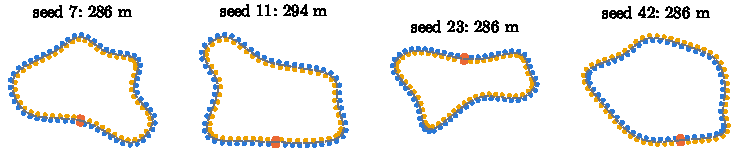
\includegraphics[width=\textwidth]{figures/dv_tracks.pdf}
\caption{Procedurally generated autocross/trackdrive layouts for four seeds (blue: left boundary, yellow: right,
orange: timing). Dashed: centre line.}
\label{fig:tracks}
\end{figure}

\subsection{Autonomous system state machine and scoring}
The AS states and mission codes match the FS Driverless CAN interface (DV system status), so they can be logged
one to one:
\begin{center}
\small Off $\to$ Ready (mission selected, ASMS on) $\to$ Driving (``Go'' after $\ge\SI{5}{s}$) $\to$ Finished
(mission complete, standstill),
\end{center}
and any active state goes to Emergency on RES, command timeout or leaving the track ($>\SI{8}{m}$ from the
centre line). Lap times are measured at timing-line crossings, interpolated within a physics sub-step. Penalties
are \SI{2}{s} per cone down and \SI{10}{s} per off-course. The skidpad times the second and fourth laps, as in the
rules. Cone contact uses the car footprint from the CAD (wing tips: $\SI{3.065}{m}\times\SI{1.48}{m}$) against the
cone base circles.

%=====================================================================================================
\section{Sensor models}\label{sec:sensors}
%=====================================================================================================
All sensors run on independent rate schedulers and publish in the car's frames and message layouts
(\cref{tab:sensors}).

\begin{table}[t]
\centering\small
\caption{Simulated sensors (\code{sensors.yaml}).}
\label{tab:sensors}
\begin{tabularx}{\textwidth}{@{}lXl@{}}
\toprule
Sensor & Model & Rate\\
\midrule
LiDAR & Ouster OS1-64, $\pm\ang{22.5}$ vertical, 1024 columns, range noise $\sigma=\SI{1.5}{cm}$, 1\,\% dropout, motion distortion; mounted on the nose ($x=\SI{1.55}{m}$, $z=\SI{0.565}{m}$) & \SI{10}{Hz}\\
Stereo camera & ZED~2i, $1280\times720$, $\ang{110}$ HFOV, baseline \SI{0.12}{m}, disparity noise \SI{0.15}{px}; on the main hoop, pitched \SI{0.12}{rad} down & \SI{15}{Hz}\\
IMU & MEMS/INS: gyro noise $1.2\times10^{-4}$\,rad/s/$\sqrt{\text{Hz}}$, accel noise $6\times10^{-4}$\,m/s$^2$/$\sqrt{\text{Hz}}$, bias random walks, optional orientation & \SI{200}{Hz}\\
GNSS & RTK fix ($\sigma_h=\SI{2}{cm}$) or single point, lever arm, ENU$\to$WGS84 & \SI{10}{Hz}\\
Vehicle & wheel speeds with slip, steering encoder, optical ground-speed sensor & \SI{100}{Hz}\\
\bottomrule
\end{tabularx}
\end{table}

\paragraph{LiDAR.} In the lite backend, every beam is ray-cast analytically against the ground plane and every
cone. A cone is modelled as an exact vertical frustum with its stripe layout, and the stripe reflectivity bands are
reproduced. The vehicle pose is interpolated per firing column across the scan, so the cloud is motion-distorted
exactly as the real sensor's. Points are in the sensor frame of their column, with the ouster-ros fields
\code{x,y,z,intensity,t,reflectivity,ring,range}; \code{ring}~0 is the top beam. In Isaac Sim the OS1 is rendered
by the RTX LiDAR model. Isaac 6.1 has no 64-channel profile, so the 128-channel profile with the same vertical FOV
is decimated to every second beam.

\paragraph{Camera.} The lite camera projects cones with the ZED intrinsics, handles occlusion by nearer cones, and
applies a range-dependent detection probability. Stereo depth noise follows the disparity error
\begin{equation}
\sigma_z = \frac{z^2\,\sigma_d}{f\,B}.
\end{equation}
In Isaac Sim, the left and right images and the renderer depth come from Replicator annotators.

\paragraph{IMU.} The specific force at the mount includes lever-arm terms,
$\vect f = \vect a + \dot{\vect\omega}\times\vect r + \vect\omega\times(\vect\omega\times\vect r) - \vect g^{b}$.
Gravity is rotated by the chassis attitude. Continuous noise densities $\sigma_c$ become discrete standard
deviations $\sigma_c\sqrt{f_s}$, and the biases follow random walks $\sigma_b\sqrt{\Delta t}$.

\paragraph{Sensor faults.} A schedule \code{<sensor>:<kind>[=value]@<start>[+<duration>]} injects the following
faults on the lite and Isaac data:
\begin{itemize}
  \item \code{dropout} and \code{freeze} (the last message repeated with new stamps);
  \item \code{latency}, LiDAR thinning, gyro bias, wheel-speed scale and GNSS jumps.
\end{itemize}

%=====================================================================================================
\section{Isaac Sim co-simulation}\label{sec:isaac}
%=====================================================================================================
\subsection{Windows--WSL link}
Isaac Sim runs on Windows and ROS~2 Jazzy runs in WSL2. NVIDIA has deprecated the DDS route between the two since
Isaac Sim~6. \code{fsdsim.link} therefore uses TCP with the framing
\begin{center}
\code{uint32 header\_len | uint32 payload\_len | JSON header | binary payload},
\end{center}
where each NumPy array in a message is moved to the payload and replaced in the JSON by
\code{\{"\_\_nd\_\_": [offset, nbytes, dtype, shape]\}}. On connect, Isaac sends a \emph{hello} with the full
configuration, then the track and the cones. Sensor frames are droppable; AS state and commands are never dropped.
All DDS traffic stays inside WSL.

\subsection{Latency analysis and fixes}
The first runs on the team PC (RTX~5060 laptop GPU, 8\,GB) showed commands up to \SI{2}{s} old and cars leaving the
track even on ground-truth cones. Instrumenting every hop gave the following causes and fixes:
\begin{enumerate}
  \item \textbf{Network path.} With WSL in mirrored networking, Isaac reached the relay over the LAN address:
        35--80\,MB/s with stalls of 0.3--\SI{0.6}{s}. The link now uses the loopback address.
  \item \textbf{Unread bulk data.} A few-kB state write blocked for \SI{0.4}{s} behind about 23\,MB/s of images
        and clouds that no node consumed. The relay now reports a \emph{sensor demand} every second, from the
        subscriber counts; without demand, Isaac sends 320-px images and 6000-point clouds.
  \item \textbf{Head-of-line blocking.} State (pose, IMU, wheels, AS) moved to a second TCP connection, so it never
        waits behind a 5\,MB camera frame. The relay skips sensor frames more than \SI{0.25}{s} older than the state
        it has already published.
  \item \textbf{Middleware load.} Full point clouds delayed \code{/clock} and odometry by up to \SI{0.4}{s} for
        every node. The dashboard now reads a 6000-point preview topic, and the full cloud is built only on demand.
  \item \textbf{Render lag.} A camera image or LiDAR scan read after a render shows the car two rendered frames
        earlier ($\approx\SI{67}{ms}$ at \SI{30}{Hz}). Stamps are shifted back by \code{frame\_lag}=2. The lag was
        measured by fitting projected labels to the cones in the images.
  \item \textbf{Driver timing.} The reference driver ticks on the wall clock, keeps only the newest odometry, and
        predicts its pose \SI{70}{ms} ahead along the arc of its last steering command.
\end{enumerate}
After the fixes, the state queueing time dropped from 0.30--\SI{0.44}{s} to at most \SI{16}{ms}, and the command age
to at most \SI{67}{ms}, with full images (\cref{tab:isaac}).

\begin{table}[t]
\centering\small
\caption{Isaac Sim runs on the team PC (11 Nov 2026), before and after the link fixes.}
\label{tab:isaac}
\begin{tabular}{@{}lcc@{}}
\toprule
& before & after\\
\midrule
State queued before sending (max) & 0.30--\SI{0.44}{s} & $\le\SI{16}{ms}$\\
Command age at the car (max) & up to \SI{2}{s} & $\le\SI{67}{ms}$\\
Trackdrive, ground truth, racing line (10 laps) & laps up to \SI{40}{s}, off track & \SI{18.85}{s}/lap, 0 cones\\
Trackdrive, fusion + SLAM, explore then race & -- & 18.82--\SI{18.88}{s}/lap, 3 cones\\
Autocross, LiDAR only (no colours) & -- & \SI{45.2}{s}, 0 cones\\
\bottomrule
\end{tabular}
\end{table}

%=====================================================================================================
\section{Perception and SLAM}\label{sec:perception}
%=====================================================================================================
No ground truth enters the perception chain. Ground truth is only used to report accuracy.

\subsection{LiDAR cone detection}
For each scan (\cref{fig:perception}, left):
\begin{enumerate}
  \item \textbf{Self-filtering.} Points inside the car's CAD outline plus a \SI{0.25}{m} margin are removed (the
        OS1 sees the nose, tyres and wings). So are points beyond \SI{25}{m} and above \SI{1.5}{m}.
  \item \textbf{Ground plane.} A plane $z=ax+by+c$ is fitted by least squares to the points within a band around
        the current estimate. The 20\,\% largest residuals are rejected and the plane is refitted, three times with
        a shrinking band (\SI{0.25}{m}$\to$\SI{0.06}{m}).
  \item \textbf{Obstacle points.} Points between \SI{0.04}{m} and \SI{0.9}{m} above the plane are kept.
  \item \textbf{Clustering.} Occupied cells of a \SI{0.15}{m} grid are joined into connected components with an
        8-neighbourhood flood fill.
  \item \textbf{Cone test.} A cluster is a cone if it has at least 3 points (2 beyond \SI{10}{m}), a horizontal
        extent of at most \SI{0.45}{m} and a height of at most \SI{0.75}{m}. Its centre is pushed
        $\SI{0.06}{m}$ along the ray, from the visible surface to the axis. A height above \SI{0.42}{m} marks a big
        orange cone.
  \item \textbf{Colour.} The reflectivity of the stripe band (30--62\,\% of the cone height) is compared with the
        body (lite backend only). The RTX LiDAR has no stripe intensities, so in Isaac the cones stay colourless
        unless the camera supplies colours.
\end{enumerate}

\subsection{Camera detection and fusion}
A YOLO11~\cite{yolo11} detector, exported to ONNX, finds cones and their colour in the ZED image. The depth image
places each cone at the lower middle of its box, pushed back by the cone radius.

\paragraph{Automatic labels.} Training labels are generated automatically. Every true cone's base plate and tip
are projected with the camera pose and intrinsics, and the depth image removes occluded cones. The camera frame
lag of \cref{sec:isaac} was found because the first labels lagged the cones at speed (mAP$_{50}$ 0.63); with
matching labels, the share of labels confirmed by depth went from 57\,\% to nearly 100\,\%.

\paragraph{Fusion.} LiDAR positions take the colour of the nearest camera detection within a gate. Matching is done
in the map frame, with each detection placed by the pose at its own stamp, over the camera frames of the last
\SI{0.8}{s}. A late camera (0.25--\SI{0.5}{s}) therefore still contributes colours.

\subsection{Landmark SLAM}
\paragraph{Prediction.} The pose is dead-reckoned from wheel speed (or ground speed) $v$, lateral speed $v_y$ and
gyro yaw rate $r$ with a midpoint rule,
\begin{equation}
\psi_m = \psi + \tfrac12 r\Delta t,\quad
\begin{bmatrix}X\\Y\end{bmatrix} \mathrel{+}= \Delta t\begin{bmatrix}\cos\psi_m & -\sin\psi_m\\ \sin\psi_m & \cos\psi_m\end{bmatrix}\begin{bmatrix}v\\ v_y\end{bmatrix},\quad
\psi \mathrel{+}= r\Delta t,
\end{equation}
and a pose history is kept. Each observed cone is put on the map with the pose at its own measurement time (a
spinning LiDAR sees cones at different times within a scan).

\paragraph{Association and correction.} Observations are associated with the nearest mapped cone within a
\SI{0.9}{m} gate. From the matches with established cones (at least three hits), the rigid transform from the
observed to the mapped positions is solved in closed form~\cite{kabsch1976}. With centred point sets $\vect a_k$
(observed) and $\vect b_k$ (mapped),
\begin{equation}
\theta = \operatorname{atan2}\!\Big(\sum_k (a_{k,x}b_{k,y} - a_{k,y}b_{k,x}),\;\sum_k (a_{k,x}b_{k,x} + a_{k,y}b_{k,y})\Big),\qquad
\vect t = \bar{\vect b} - R(\theta)\,\bar{\vect a}.
\end{equation}
A fraction $g=0.5$ of $(\vect t,\theta)$ is applied to the pose, the history and the observations. Fits with
$|\theta|>\SI{0.1}{rad}$ or $\lVert\vect t\rVert>\SI{1}{m}$ are rejected as wrong associations.

\paragraph{Map update.} Matched landmarks are updated by a running mean with weight $1/\min(n+1, 30)$, and their
colour by voting. Unmatched observations start candidates, which must be confirmed three times within \SI{2}{s}.
Loop closure needs no special step as long as the drift over a lap stays inside the gate.

\paragraph{A fresh pose for the controller.} The SLAM pose reached the driver 0.15--\SI{0.27}{s} after its stamp in
Isaac Sim. The driver therefore integrates wheel speeds and gyro itself, and takes from SLAM only the slowly varying
correction (the map$\to$odom offset at the SLAM stamp, as in ROS navigation). The perception node processes
odometry, camera and scans in stamp order, holding messages back for at most \SI{0.1}{s}. Out-of-order execution had
caused a \SI{0.8}{m} drift per lap.

\begin{figure}[t]
\centering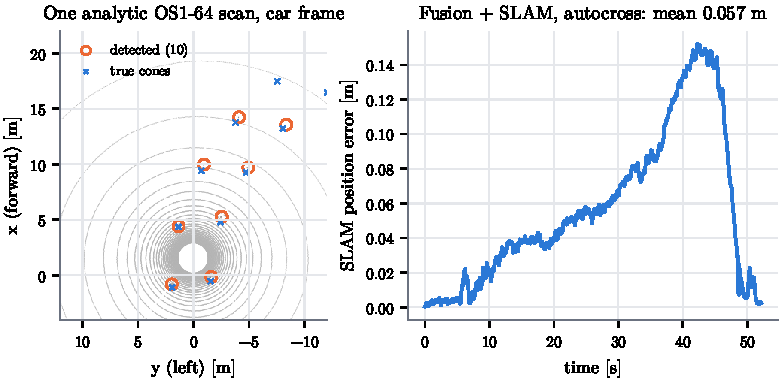
\includegraphics[width=\textwidth]{figures/dv_perception.pdf}
\caption{Left: one analytic OS1-64 scan in the car frame (grey, by height) with the detected cones (circles) and
the true cones (crosses). Right: SLAM position error during an autocross run with LiDAR--camera fusion and SLAM in
the lite backend.}
\label{fig:perception}
\end{figure}

%=====================================================================================================
\section{Control}\label{sec:control}
%=====================================================================================================
\subsection{Reference driver}
The reference driver closes the loop until the team's own stack replaces it.

\paragraph{Steering.} Pure pursuit~\cite{coulter1992} steers the rear axle towards a target point at look-ahead
distance $l_d$ on the reference path. With the target in the vehicle frame at $(l_x, l_y)$,
\begin{equation}
\delta = \operatorname{sat}_{\pm\delta_{\max}}\operatorname{atan2}\!\big(2L\,l_y,\; l_x^2 + l_y^2\big),\qquad
l_d = \min\!\Big(\operatorname{clip}(0.30\,v + 3, 3, 9),\; \max\big(2,\, 0.45/\kappa_{\max}\big)\Big),
\label{eq:pp}
\end{equation}
where $\kappa_{\max}$ is the largest path curvature within the look-ahead, which keeps the driver from cutting
tight corners. Two compensations are applied:
\begin{itemize}
  \item a steering preview of \SI{0.05}{s}, for actuator lag and control period;
  \item an optional pose prediction along the arc of the last steering command over the known latency
        (\SI{70}{ms} in Isaac Sim, without which the skidpad failed from the third lap).
\end{itemize}

\paragraph{Speed.} The target speed profile $v_{ref}(s)$ is the QSS speed profile of the \emph{running car} on the
reference path~\cite{perflab}, computed at grip utilisation $u_g=0.8$. Braking additionally uses only 70\,\% of the
longitudinal grip. The point-mass QSS model does not see the rear axle unloading under braking, and braking earlier
keeps the car stable. The command is
\begin{equation}
a_c = \operatorname{clip}\big(k_p\,(v_t - v),\, -a_{dec},\, a_{acc}\big),\qquad
v_t = \min\big(v_{ref}(s),\, v_{ref}(s + 0.4\,v)\big),
\end{equation}
with $k_p=2.5\,\si{s^{-1}}$. After the finish, the car brakes firmly on straights and gently in corners
(deceleration reduced with lateral acceleration), and never faster than the profile allows.

\paragraph{Cones mode.} With only perceived cones, a local planner pairs blue and yellow boundaries into a centre
path. Cones without colour are assigned by following each boundary cone by cone (next cone 1--\SI{7}{m} on, turning
at most \ang{70}), and big orange cones near the car stand in for the boundaries at the timing line. This lets
autocross and trackdrive finish with no colour information at all. With \code{race\_after=N}, the driver explores
for $N$ laps, then drives the mapped track (centre or racing line) at the limits of the car.

\subsection{Racing line}
The racing line moves the centre line $\vect c$ sideways by offsets $\vect a$ along fixed normals $N$, bounded by
the half width minus half the car width minus a margin. Curvature and length are then linear in $\vect a$, so the
line is the solution of a bounded least-squares problem,
\begin{equation}
\min_{\vect a}\; \lVert D_2(\vect c + N\vect a)\rVert^2 + w\,\lVert D_1(\vect c + N\vect a)\rVert^2\quad
\text{s.t.}\; -\vect b\le\vect a\le\vect b,
\end{equation}
solved by active-set iterations. The weight $w=0$ gives minimum curvature; a large $w$ gives the shortest path. The
car's own QSS model picks the fastest of a few $w$. On the generated circuits the QSS gain is about 6\,\%. Driven
by the reference driver it is 2--3\,\% (seed~7: \SI{20.12}{s}$\to$\SI{19.48}{s},
\cref{fig:closedloop}).

\begin{figure}[t]
\centering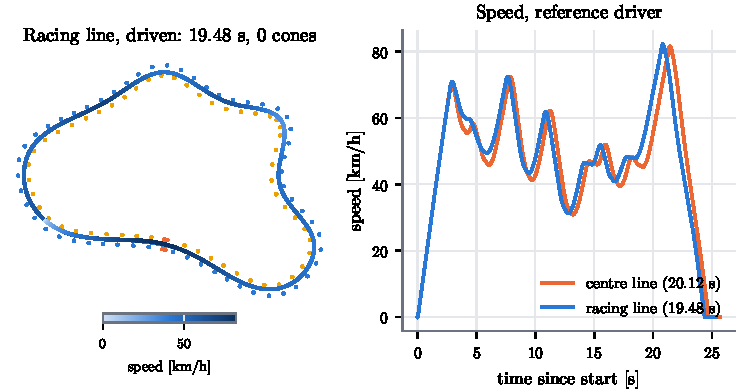
\includegraphics[width=\textwidth]{figures/dv_closedloop.pdf}
\caption{Closed-loop autocross on layout seed~7, map mode, reference driver. Left: the driven racing line coloured
by speed. Right: speed over time for the centre and racing lines.}
\label{fig:closedloop}
\end{figure}

\subsection{Learned longitudinal control}
Steering stays with pure pursuit; the policies only control throttle and brake.

\paragraph{Per-setup policy.} A multilayer perceptron (26$\to$32$\to$32$\to$1, $\tanh$) receives the following
inputs:
\begin{itemize}
  \item the speed;
  \item the QSS limit speed and the path curvature at eight look-ahead distances (0--\SI{60}{m});
  \item lateral velocity, yaw rate, accelerations and sideslip;
  \item the tracking errors and the previous action.
\end{itemize}
It outputs $a\in[-1,1]$, scaled to the throttle or brake limit. Training starts with DAgger imitation of the
reference driver~\cite{ross2011} (four rounds). OpenAI evolution strategies~\cite{salimans2017} then optimise the
output layer on headless \code{fsdsim} runs.

\paragraph{Universal policy.} \code{fsdsim.vec} re-implements the performance-mode vehicle, pure pursuit, cone
contact and timing as array code for $N$ cars with $N$ specifications, on NumPy or PyTorch/CUDA. The trajectories
equal those of \code{fsdsim} to $10^{-9}$\,m. PPO~\cite{schulman2017,schulman2016} trains one policy over a range of
specifications:
\begin{itemize}
  \item mass $\times0.85$--1.15, friction $\times0.85$--1.12, $c_z$ $\times0.7$--1.3;
  \item power 40--\SI{80}{kW}, RWD or AWD, and more.
\end{itemize}
The policy is \emph{told} the specification: 15 numbers, plus a speed envelope computed from the car's own LapSim
limits. Hidden domain randomisation keeps a driver's margin:
\begin{itemize}
  \item grip $\times0.95$--1.03;
  \item actuator lags $\times0.8$--1.4;
  \item a latency of 0 or \SI{40}{ms}, and sensor noise.
\end{itemize}
The reward is metres of progress, $-30$ per cone, and $-100$ (ending the episode) for leaving the track. On held-out
tracks and setups, the universal policy scores 7.4\,\% better than the reference speed law, 9.4\,\% on autocross,
with fewer cones (12 against 22 in 90 runs). \Cref{tab:rl} lists complete missions in the full simulator.

\begin{table}[t]
\centering\small
\caption{Complete missions in the full simulator: reference driver against the universal RL policy (official
timing; all RL runs clean). Reference values predate the steering preview of 9 Nov 2026.}
\label{tab:rl}
\begin{tabular}{@{}llcc@{}}
\toprule
Setup & Mission & Reference driver & Universal RL\\
\midrule
LapSim baseline & Acceleration & \SI{4.767}{s} & \textbf{\SI{4.387}{s}}\\
& Skidpad & \SI{5.494}{s} & \textbf{\SI{5.392}{s}}\\
& Trackdrive, 10 laps (layout 7) & \SI{197.05}{s} & \textbf{\SI{183.09}{s}}\\
$m=\SI{260}{kg}$, $c_z=4.6$ & Acceleration / skidpad & 4.655 / \SI{5.432}{s} & \textbf{4.212 / \SI{5.256}{s}}\\
AWD, \SI{60}{kW}, $\mu\times0.92$ & Autocross layout 7 & \SI{20.41}{s} +3 cones +1 OC & \textbf{\SI{18.68}{s}}, clean\\
\bottomrule
\end{tabular}
\end{table}

%=====================================================================================================
\section{Verification}\label{sec:verification}
%=====================================================================================================
The project is verified at four levels:
\begin{enumerate}
  \item \textbf{Unit tests (319).} They cover the LapSim port against the team's MATLAB results (largest
        difference below \SI{0.005}{ms} over 85 parameter values and all four events), the vehicle model, sensors,
        perception, SLAM, the link protocol, the batched model (NumPy and PyTorch equal, trajectories equal to
        \code{fsdsim}), the dashboard, the launcher and the Performance Lab.
  \item \textbf{Closed-loop regression.} \code{tools/regression.py} runs 33 cases: all events at 50 and \SI{20}{Hz}
        driver rates, four circuits on centre and racing line, double track, perception with SLAM, and sensor
        faults. It must pass before and after any model or driver change.
  \item \textbf{Offline reproduction of PC defects.} Every timing defect seen on the team PC was first reproduced
        without Isaac Sim (e.g.\ command latency, out-of-order messages), so the fix is covered by a test.
  \item \textbf{Team-PC test plan.} The items that need Isaac Sim, MATLAB or the GPU follow a written test plan
        with expected values.
\end{enumerate}

%=====================================================================================================
\section{Results}\label{sec:results}
%=====================================================================================================
\paragraph{Events with the reference driver.} With ground-truth cones and the default driver at \SI{50}{Hz}, every
event finishes with 0 cones and 0 off-course:
\begin{itemize}
  \item acceleration in \SI{4.77}{s} (LapSim \SI{4.66}{s});
  \item skidpad in \SI{5.375}{s} (LapSim \SI{5.154}{s});
  \item autocross on layout~7 in exploration (cones) mode in \SI{44.81}{s}, and in map mode in \SI{20.12}{s} on the
        centre line and \SI{19.48}{s} on the racing line;
  \item trackdrive with ten laps of \SI{44.78}{s} in exploration mode.
\end{itemize}
The gaps to LapSim come from the driver's grip margin and the yaw, actuator and tracking dynamics that the QSS
model does not have.

\paragraph{Perception and SLAM.} In the lite backend with LiDAR--camera fusion and SLAM (no ground truth to the
driver), the autocross on layout~7 finishes in \SI{43.21}{s} with 0 cones. All 113 cones are mapped with no false
cones. The cone position error is \SI{0.074}{m} rms (max \SI{0.150}{m}), the SLAM pose error averages \SI{0.057}{m}
(max \SI{0.152}{m}), and the heading error stays below \ang{0.28} (\cref{fig:perception}). In Isaac Sim, the SLAM
pose is 0.2--\SI{0.4}{m} off. The RTX LiDAR cones scatter 0.08--\SI{0.15}{m} around the truth (lite: 0.01--0.03),
and no systematic offset or timing error remains.

\paragraph{Sensitivities: simulator against LapSim.} \Cref{tab:sens} compares the time sensitivities of the
closed-loop simulator with those of LapSim (central differences over $\pm10\,\%$). The two models agree in sign
and order. Grip matters slightly more to the driverless car on autocross, and mass and gear ratio matter less,
because the driver is not at the traction or power limit most of the lap. Acceleration does not respond to grip in
either model: the LR26 is motor-limited for 85--100\,\% of the run.

\begin{table}[t]
\centering\small
\caption{Time sensitivity [s per +1\,\% of the parameter], LapSim (QSS) against the closed-loop simulator
(\code{param\_study.py --table}; autocross on the simulator's own layout).}
\label{tab:sens}
\begin{tabular}{@{}lrrrrrr@{}}
\toprule
& \multicolumn{2}{c}{Acceleration} & \multicolumn{2}{c}{Skidpad} & \multicolumn{2}{c}{Autocross}\\
\cmidrule(lr){2-3}\cmidrule(lr){4-5}\cmidrule(l){6-7}
Parameter & LapSim & Sim & LapSim & Sim & LapSim & Sim\\
\midrule
$\mu$ ($x$ and $y$) & 0.000 & $-0.006$ & $-0.028$ & $-0.029$ & $-0.083$ & $-0.093$\\
$m$ & $+0.022$ & $+0.015$ & $+0.005$ & $+0.004$ & $+0.038$ & $+0.026$\\
$i$ & $-0.024$ & $-0.018$ & 0.000 & 0.000 & $-0.025$ & $-0.014$\\
$h$ & 0.000 & 0.000 & $+0.001$ & $+0.001$ & $-0.001$ & 0.000\\
$c_z$ & 0.000 & 0.000 & $-0.002$ & $-0.002$ & $-0.008$ & $-0.009$\\
$c_w$ & $+0.001$ & $+0.002$ & 0.000 & $+0.001$ & $+0.002$ & $+0.003$\\
\bottomrule
\end{tabular}
\end{table}

%=====================================================================================================
\section{Limitations and future work}\label{sec:limits}
%=====================================================================================================
\begin{itemize}
  \item \textbf{Identification.} Chassis attitude parameters, actuator lags, yaw inertia and the tyre shape
        $(B,C,E)$ are typical values, not measured on the LR26. The next step towards a digital twin is fitting
        them to coast-down, step-steer, skidpad and acceleration logs. The team's only car log so far has no GPS,
        IMU or wheel speeds.
  \item \textbf{Model scope.} Suspension kinematics, tyre temperature and tyre transients are not modelled. Torque
        vectoring is possible with double track but not implemented.
  \item \textbf{Perception.} The YOLO detector is trained on simulator images. Real images (e.g.\ FSOCO) must be
        added for the car. The SLAM has no covariance or global optimisation, and a gyro bias of
        \SI{0.02}{rad/s} moves it by metres.
  \item \textbf{GPU training.} The batched model launches many small GPU kernels, so 4096 cars on an RTX~5060 run
        at about 4400 steps/s, no faster than one CPU core. The Isaac Lab training path has not been run yet.
  \item \textbf{Hardware in the loop.} The simulator already speaks the DV logging CAN frames. A bridge to the
        team's VCU messages would allow testing the real computer.
\end{itemize}

%=====================================================================================================
\section{Conclusion}
%=====================================================================================================
fsg-dv-sim shows that a Formula Student driverless simulator can share its vehicle with the performance group's
lap time simulation without losing the dynamics needed for control development. Keeping behaviour in one GPU-free
core, and treating the renderer as an exchangeable sensor source, made it possible to:
\begin{itemize}
  \item verify most of the system with ordinary unit tests;
  \item reproduce timing defects of the GPU co-simulation offline;
  \item train learned controllers on thousands of vehicle variants with the same physics.
\end{itemize}
The open items are data, not code: identified chassis and tyre parameters, real camera images and calibrated
sensor noise.

%=====================================================================================================
\begin{thebibliography}{99}\small
\bibitem{perflab} Lions Racing Team, ``Performance Lab: quasi-steady-state and transient lap time simulation of
the LR26 Formula Student vehicle,'' technical report, Nov.~2026 (companion report, \code{docs/paper}).
\bibitem{fssim} AMZ Driverless, ``FSSIM: Formula Student Simulator,'' software, ETH Zürich, 2018.
\bibitem{kabzan2020} J.~Kabzan \emph{et al.}, ``AMZ Driverless: The full autonomous racing system,''
\emph{Journal of Field Robotics}, vol.~37, no.~7, pp.~1267--1294, 2020.
\bibitem{rajamani2012} R.~Rajamani, \emph{Vehicle Dynamics and Control}, 2nd~ed. Springer, 2012.
\bibitem{pacejka2012} H.~B.~Pacejka, \emph{Tire and Vehicle Dynamics}, 3rd~ed. Butterworth-Heinemann, 2012.
\bibitem{siegler2000} B.~Siegler, A.~Deakin, D.~Crolla, ``Lap time simulation: Comparison of steady state,
quasi-static and transient racing car cornering strategies,'' SAE Technical Paper 2000-01-3563, 2000.
\bibitem{brayshaw2005} D.~L.~Brayshaw, M.~F.~Harrison, ``A quasi steady state approach to race car lap simulation
in order to understand the effects of racing line and centre of gravity location,'' \emph{Proc.\ IMechE Part~D:
J.\ Automobile Engineering}, vol.~219, no.~6, pp.~725--739, 2005.
\bibitem{casanova2000} D.~Casanova, ``On minimum time vehicle manoeuvring: The theoretical optimal lap,''
PhD thesis, Cranfield University, 2000.
\bibitem{heilmeier2020} A.~Heilmeier \emph{et al.}, ``Minimum curvature trajectory planning and control for an
autonomous race car,'' \emph{Vehicle System Dynamics}, vol.~58, no.~10, pp.~1497--1527, 2020.
\bibitem{coulter1992} R.~C.~Coulter, ``Implementation of the pure pursuit path tracking algorithm,'' Carnegie
Mellon University, Tech.\ Rep.\ CMU-RI-TR-92-01, 1992.
\bibitem{dhall2019} A.~Dhall, D.~Dai, L.~Van~Gool, ``Real-time 3D traffic cone detection for autonomous driving,''
in \emph{Proc.\ IEEE Intelligent Vehicles Symposium}, 2019.
\bibitem{yolo11} G.~Jocher, J.~Qiu, ``Ultralytics YOLO11,'' software, 2024.
\bibitem{kabsch1976} W.~Kabsch, ``A solution for the best rotation to relate two sets of vectors,''
\emph{Acta Crystallographica A}, vol.~32, no.~5, pp.~922--923, 1976.
\bibitem{ross2011} S.~Ross, G.~Gordon, D.~Bagnell, ``A reduction of imitation learning and structured prediction to
no-regret online learning,'' in \emph{Proc.\ AISTATS}, 2011.
\bibitem{salimans2017} T.~Salimans, J.~Ho, X.~Chen, S.~Sidor, I.~Sutskever, ``Evolution strategies as a scalable
alternative to reinforcement learning,'' arXiv:1703.03864, 2017.
\bibitem{schulman2017} J.~Schulman, F.~Wolski, P.~Dhariwal, A.~Radford, O.~Klimov, ``Proximal policy optimization
algorithms,'' arXiv:1707.06347, 2017.
\bibitem{schulman2016} J.~Schulman, P.~Moritz, S.~Levine, M.~Jordan, P.~Abbeel, ``High-dimensional continuous
control using generalized advantage estimation,'' in \emph{Proc.\ ICLR}, 2016.
\bibitem{makoviychuk2021} V.~Makoviychuk \emph{et al.}, ``Isaac Gym: High performance GPU-based physics simulation
for robot learning,'' arXiv:2108.10470, 2021.
\bibitem{mittal2023} M.~Mittal \emph{et al.}, ``Orbit: A unified simulation framework for interactive robot
learning environments,'' \emph{IEEE Robotics and Automation Letters}, vol.~8, no.~6, pp.~3740--3747, 2023.
\bibitem{macenski2022} S.~Macenski, T.~Foote, B.~Gerkey, C.~Lalancette, W.~Woodall, ``Robot Operating System 2:
Design, architecture, and uses in the wild,'' \emph{Science Robotics}, vol.~7, no.~66, 2022.
\end{thebibliography}

%=====================================================================================================
\appendix
\section{Reproducing the results}
\begin{itemize}[before=\sloppy]
  \item Figures and the numbers quoted here: \code{python3 docs/paper/figures/make\_figures.py}, which also writes
        \code{numbers.json}.
  \item Unit tests: \code{python3 -m unittest discover -s tests}.
  \item Closed-loop runs: \code{python3 tools/closed\_loop\_eval.py --strict} and \code{python3 tools/regression.py}.
  \item Perception run of \cref{fig:perception}:
        \code{python3 tools/closed\_loop\_eval.py --mission autocross --perception fusion --slam}.
\end{itemize}

\section{ROS 2 interface (selection)}
\begin{center}\small
\begin{tabular}{@{}ll@{}}
\toprule
Topic & Content\\
\midrule
\code{/lidar/points} & \code{PointCloud2}, ouster-ros fields\\
\code{/zed/zed\_node/left/image\_rect\_color}, \code{.../depth} & ZED wrapper layout\\
\code{/imu/data}, \code{/gnss/fix}, \code{/vehicle/sensors} & proprioceptive sensors\\
\code{/as/status} & AS state, mission, laps, penalties\\
\code{/control/command} & steering and acceleration request (watchdog)\\
\code{/perception/cones}, \code{/slam/odom} & perception output\\
\code{/ground\_truth/*} & evaluation only\\
\bottomrule
\end{tabular}
\end{center}

\end{document}
